\documentclass[11pt,fullpage]{article}
\usepackage{fullpage}
\usepackage{graphicx}
\usepackage{times}
\usepackage{cite}
\usepackage{listings}
\linespread{1}

\begin{document}
\author{W. Trimble}
\date{Feb 27 2014 (v0.9)}
\title{Using \texttt{kmerspectrumanalyzer} }
\maketitle
\bibstyle{apsrev}
\section{Background}
$k$-mers (also called ($\ell$-tuples, $n$-grams, and occasionally ``words'') are
subsets of a sequence of fixed length that are used for the analysis and
interpretation of sequence data.   

Li and Waterman noticed in 2003 that a genome of size $G$ generates about $G$ distinct
long kmers, despite the overlapping nature of their construction and the reverse-complement
degeneracy.

The tables of numbers summarizing how many kmers have been seen exactly $n$ times 
are produced by and used by a number of bioinformatics tools, particularly assemblers,
but presenting the spectra in a way that makes the underlying 
facts about sequencing depth and sequence diversity plain has been a challenge.

\texttt{kmerspectrumanalyzer} is a collection of scripts to facilitate the counting of 
kmers in large datasets and to make sense of the otherwise very abstract and dry tables
of numbers that pass for kmer spectra.  

\section{Installation}
\subsection{Get kmerspectrumanalyzer} 
To get \texttt{kmerspectrumanalyzer}, use \texttt{git} to clone the repository:
%\begin{lstlisting}
\begin{verbatim}
git clone http://github.com/MG-RAST/kmerspectrumanalyzer.git
\end{verbatim}

\subsection{Dependencies} 
The script \texttt{testdependencies.sh} tests for missing dependencies and 
offers suggestions of how to install them.    

A script preparing a blank EC2 nodes is in \texttt{src/setup\_environment.sh}. 
\begin{verbatim}
sudo apt-get install -y jellyfish python-matplotlib python-scipy
\end{verbatim}
are sufficient to prepare the python environment.  

\begin{tabular}{llrrr}
&\\
Package & Source \\
  \texttt{git}  &    \texttt{http://git-scm.com/downloads}\\
  \texttt{python} ($>$v2.6)  &    \texttt{http://python.org}\\
  \texttt{numpy} & \texttt{http://www.numpy.org/} \\
  \texttt{scipy} &  \texttt{http://www.scipy.org/} \\
   \texttt{matplotlib} & \texttt{http://www.matplotlib.org/}\\
   \texttt{jellyfish} (v1.15) & \texttt{http://www.cbcb.umd.edu/software/jellyfish/} \\
&\\
\end{tabular}

\section{Input and output data}
The first step in analyzing kmers is to count the kmers in a dataset
or a subset of a sequence dataset in fasta or fastq formats.
Ambiguous bases in the input are ignored and are not counted. 
Raw sequence data from Illumina, 454, and Iontorrent sequencing machines can
be counted if they can be converted to FASTQ formats. 
(In principle the analysis should work for colorspace data, but this requires
double-encoding and hasn't been tested.)   
Kmer counts of assemblies or collections of genomes make sense, too. 
\texttt{countkmer21.sh} invokes \texttt{kmer-tool2} which invokes
\texttt{jellyfish} to count the kmers.  

\begin{tabular}{lll}
&&\\
\hline
Program & Input  & Output \\
\texttt{countkmer21.sh}          &  FASTA or FASTQ               &  kmer spectrum \\ 
\texttt{plotkmerspectrum.py}     & 1 or more kmer spectra        & graphs, kmer statistics \\
                                 & or list of spectrum files     &  \\
\texttt{kmerspectrumanalyzer.py} & kmer spectrum                 & fit parameters  \\ 
\hline
&&\\
\end{tabular}

The default output is a table of 
integers, called the kmer spectrum.  Table \ref{kmerspectrum} illustrates what the kmer spectrum
looks like.  Pretty dull.   Note: this table is much smaller than the sequence data it summarizes,
and contains none of the sequences, only the histogram of kmer redundancies.  

\begin{table}
\begin{tabular}{rrrrr}
1 & 19017971 & There are 19 million unique 21-mers in this dataset \\
2 & 1285011  & followed by 1.3 million 21-mers with exactly 2 copies \\
3 & 323553  \\
4 & 134192  \\
5 & 68913  \\
10 & 8380  & ... and 8380 21-mers that were present 10 times each \\
20 & 1225  \\
30 & 3172  \\
40 & 12354  \\
50 & 57350  \\
60 & 138218 & \\
70 & 143173 & the mode in the kmer spectrum is around here \\
80 & 71551  \\
90 & 20826  \\
100 & 4104  \\
200 & 91  \\
400 & 26  \\
. & . \\
5172 & 1 & at high abundances, the spectrum invariably becomes sparse \\
5256 & 1  \\
5323 & 1  \\
17265 & 1 &  This is the most abundant 21-mer in this dataset \\
\end{tabular}
\caption{Table of the 21-mer spectrum for SRR001665 - E. coli genomic sequencing - in \texttt{SRR001665-both.21} }
\label{kmerspectrum}
\end{table}

To generate spectra, first download some sequencing data.  
PRJNA30551 / SRX000429 / SRR001665  is an illumina run sequencing our friend E. coli.

A script downloading SRR001665\_1.fastq.gz and SRR001665\_1.fastq.gz from ERA is in test/workflow-example.sh.
%\begin{verbatim}
%curl ftp://ftp.sra.ebi.ac.uk/vol1/fastq/SRR001/SRR001665/SRR001665_1.fastq.gz > SRR001665_1.fastq.gz
%curl ftp://ftp.sra.ebi.ac.uk/vol1/fastq/SRR001/SRR001665/SRR001665_2.fastq.gz > SRR001665_2.fastq.gz
%\end{verbatim}

Streaming the files to \texttt{countkmer21.sh} will count the 21-mers and give us a summary table:
\begin{verbatim}
zcat SRR001665_1.fastq.gz | countkmer21.sh > SRR001665_1.21
\end{verbatim}

We can count kmers in both the forward and reverse reads at once by streaming both files:
\begin{verbatim}
zcat SRR001665_*.fastq.gz | countkmer21.sh > SRR001665-both.21
\end{verbatim}

If we have uncompressed files, \texttt{countkmer21.sh} will take one or more sequence filenames:
\begin{verbatim}
gunzip SRR001665_2.fastq.gz
countkmer21.sh SRR001665_2.fastq 
\end{verbatim}
At this point we have created three spectrum files: SRR001665\_1.fastq.21,  SRR001665\_2.fastq.21,  and SRR001665-both.21.

The following commands make graphs of the all-data spectrum: 
\begin{verbatim}
plotkmerspectrum.py SRR001665-both.21  -w png -g 1
plotkmerspectrum.py SRR001665-both.21  -w png -g 5
plotkmerspectrum.py SRR001665-both.21  -w png -g 6
\end{verbatim}
This creates several image files with graphs of the spectrum, named like \texttt{SRR001665-both.21.5.png}.
Each run of plotkmerspectrum also appends a line containing summary statistics of the kmer spectrum,
described in table \ref{statisticstable}.

\begin{verbatim}
kmerspectrumanalyzer.py SRR001665-both.21
\end{verbatim}

\begin{table}
\begin{tabular}{rrl}
field name & value & Description \\
\hline 
filename	 & SRR001665-both.21 & Name of file summarized \\
M10  & 300236	 & Minimum number of kmers to explain 10\% of data\\
M50  & 2084233	 & Minimum number of kmers to explain 50\% of data \\
M90  & 4331807	 & Minimum number of kmers to explain 90\% of data \\
M100 & 25506196	 & Number of unique kmers  (explains 100\% of data)\\
F100 & 0.000720	 & Fraction of data in first 100 kmers\\
F10K & 0.015142	 & Fraction of data in first 10K kmers \\
F1M &  0.267744 &  Fraction of data in first 1M kmers  \\
H & 6329205.6	 &  antilog-Shannon entropy of kmer distribution \\
H2 & 4483639.5	 &  Reyni entropy (reciprocal Simpson index)  \\
AVC & 74.0	 &  Mean coverage  (unreliable) \\
AVG & 1198148.5	 &   Observation-weighted "genome size" (unreliable)\\
C50 & 68.0       &   Observation-weighted median coverage  \\
\hline 
\end{tabular}
\caption{Kmer spectrum summary statistics, calculated by \texttt{plotkmerspectrum.py} } 
\label{statisticstable}
\end{table}

The first step, counting the kmers, is the most expensive step; it requires 
hard drive space sufficient for a duplicate copy of the data and was tested
and optimized on servers with 8Gb of memory.  After the kmers have been
counted, the resulting spectra are small (few tens of kbyte) summaries of
the kmer redundancy, and the subsequent scripts (kmerspectrumanalyzer,
plotkmerspectrum) do not require extraordinary compute resources and
can run on desktop machines.


\begin{figure}
\begin{tabular}{lll}
\hline
file &     SRR001665-both.21 & filename \\
cmd   &  kmerspectrumanalyzer.py &  command summary\\ 
cov   &  66.4                   & fitted first peak abundance \\
shape &  0.02                   & shape parameter \\
gsize &  4580543.8              & genome size  estimate \\
ngthalf & 4515807               & number of kmers above cov/2 \\ 
1     &  4468388.5              & kmers in peak at cov \\
2     &  13663.1                & kmers in peak at cov * 2 \\
3     &  5449.5                 & ... \\
4     &  2693.0 &  \\
5     &  1600.6 &  \\
6     &  1296.4 &  \\
7     &  2848.4 &  \\
8     &  2166.1 &  \\
9     &  147.3  &  \\
10    &  333.4  &  \\
sumerr & 19269.971407 & Value of the score function \\
\hline
\end{tabular}
\caption{Contents of \texttt{SRR001665-both.21.fit.csv}, table of fit coefficients for the mixed-Poisson model.  
This fit predicts a 4.58 Mbase genome at abundance 66x.}
\end{figure}

\section{Visualizations}
\subsection{Plain kmer spectrum (graph 0)}
% \begin{figure}
% \begin{center}
% \includegraphics[width=3in]{graphs/nicelist0.pdf}
% \end{center}
% \caption{Plain kmer spectrum}
% \end{figure}
The kmer spectrum is the plot of number of distinct kmers observed vs. the number of 
occurrences of each (the abundance)--the result of directly plotting the kmer
spectrum table.  This graph is the simplest but is neither the 
prettiest nor the most useful.  This graph puts rare kmers on the left and
abundant kmers on the right.  The high-abundance end of the graph does not render well
because of the low occupancy of the histogram at high abundances -- at a high enough
abundance the histogram is likely to bounce between abundance values that have 0 
occurrences and nearby values that have only 1. 

\subsection{Observed kmers spectrum (graph 1) }

This spectrum is a minor modification of the plain kmer spectrum in which the number
of kmers has been multiplied by the abundance to give number of observed kmers.
The resulting shapes are more beautiful. 

\begin{figure}
\begin{center}
\includegraphics[width=3in]{graphs3/SRR001665-both-21-1.pdf} 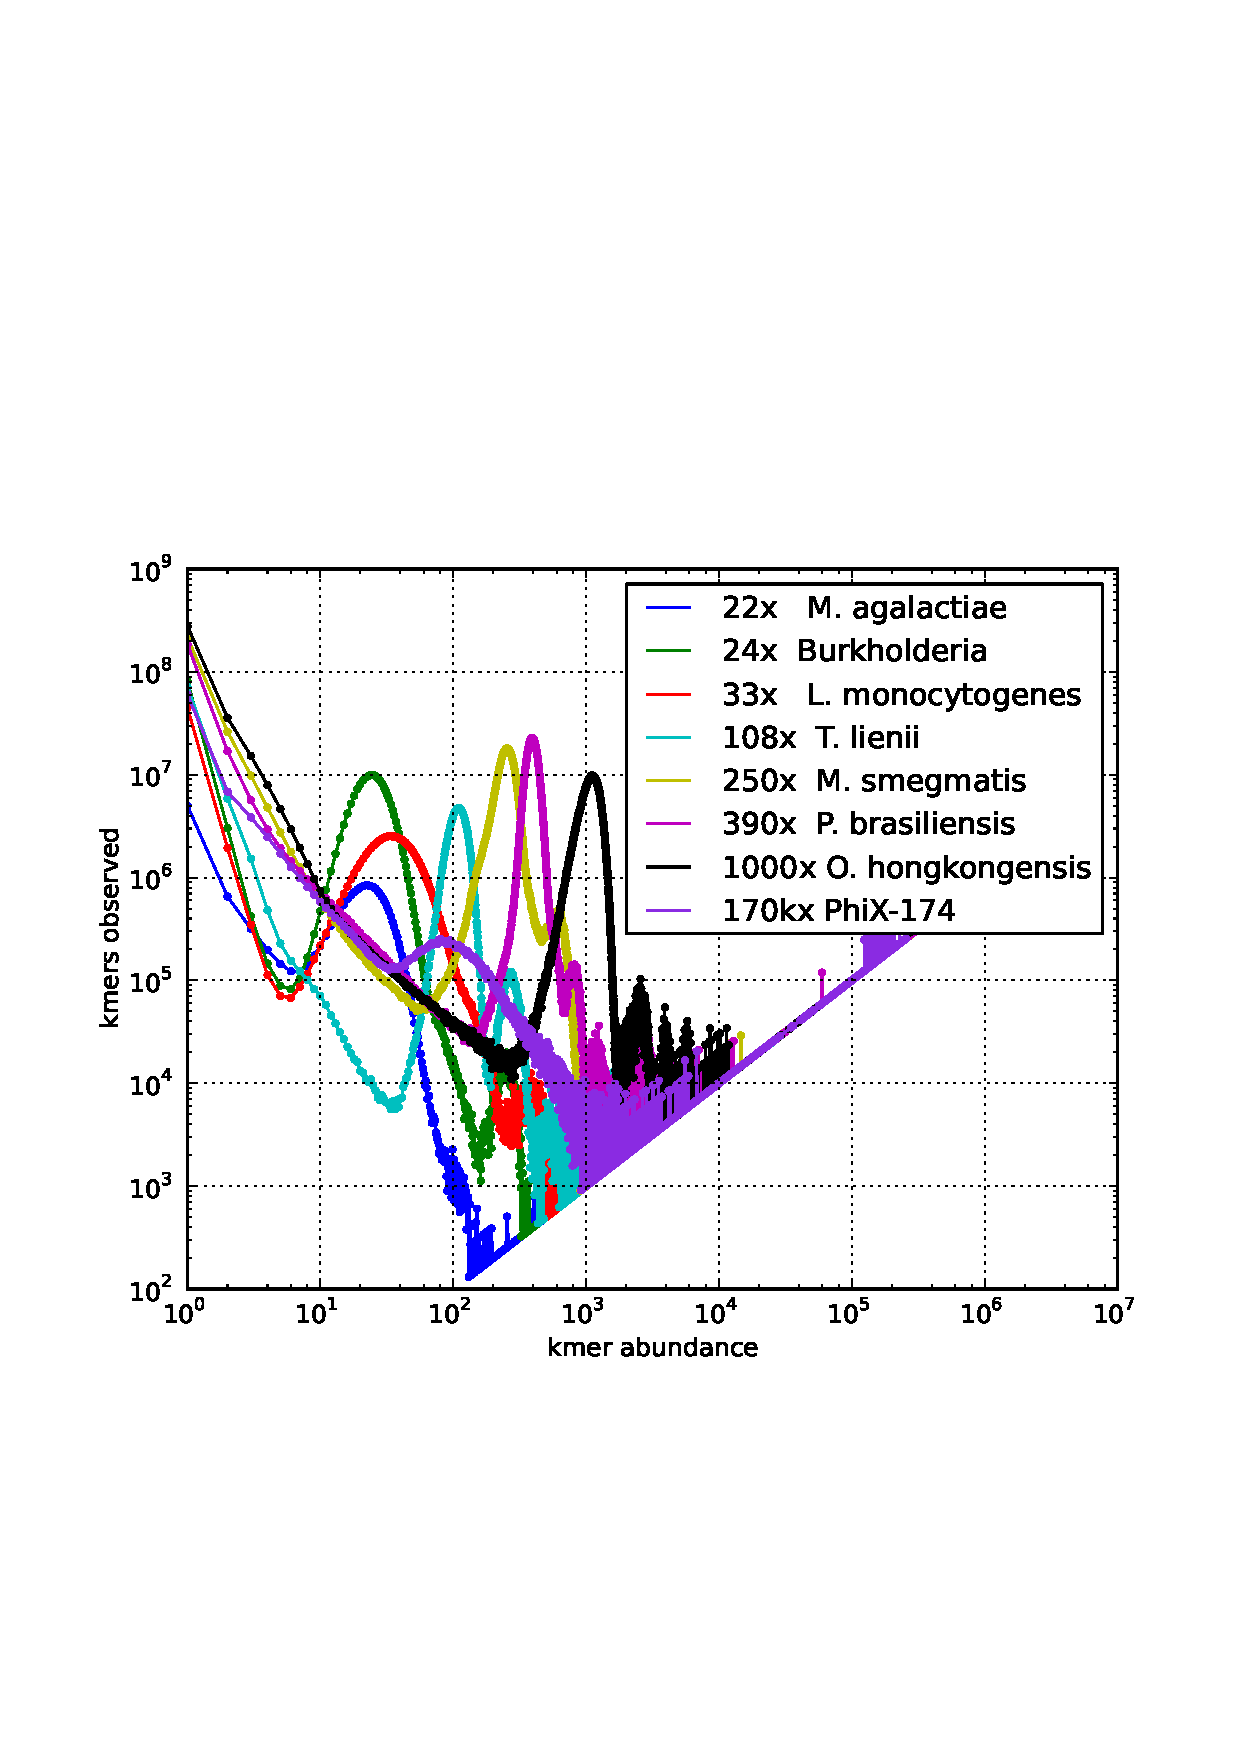
\includegraphics[width=3in]{graphs2/filelistcv-1.pdf}
\end{center}
\caption{Observed kmer spectrum (graph 1).  E. coli is on the left, various genomes are compared on the right.  
Rare kmers appear on the left, while abundant kmers appear on the right (and are obscured by graphing and sampling artifacts) 
The first point on the left represents unique kmers; the leftmost several points are "nonsolid" kmers
that are presumptive sequencing errors. }
\label{graph1}
\end{figure}

\subsection{Ranked kmers consumed (graph 5) }

Ranking the kmers from most abundant to least abundant, they have the property that the 
first $n$ kmers always explain more of the dataset than any other set of the same number
of kmers.  Progressing from the most redundant (highest abundance) to least redundant 
(unique) sequences in the dataset takes us from the left side of the graph to the right, 
with the x-axis counting the total (cumulative) number of the highest-abundance kmers.

\begin{figure}
\begin{center}
\includegraphics[width=3in]{graphs3/SRR001665-both-21-5.pdf} 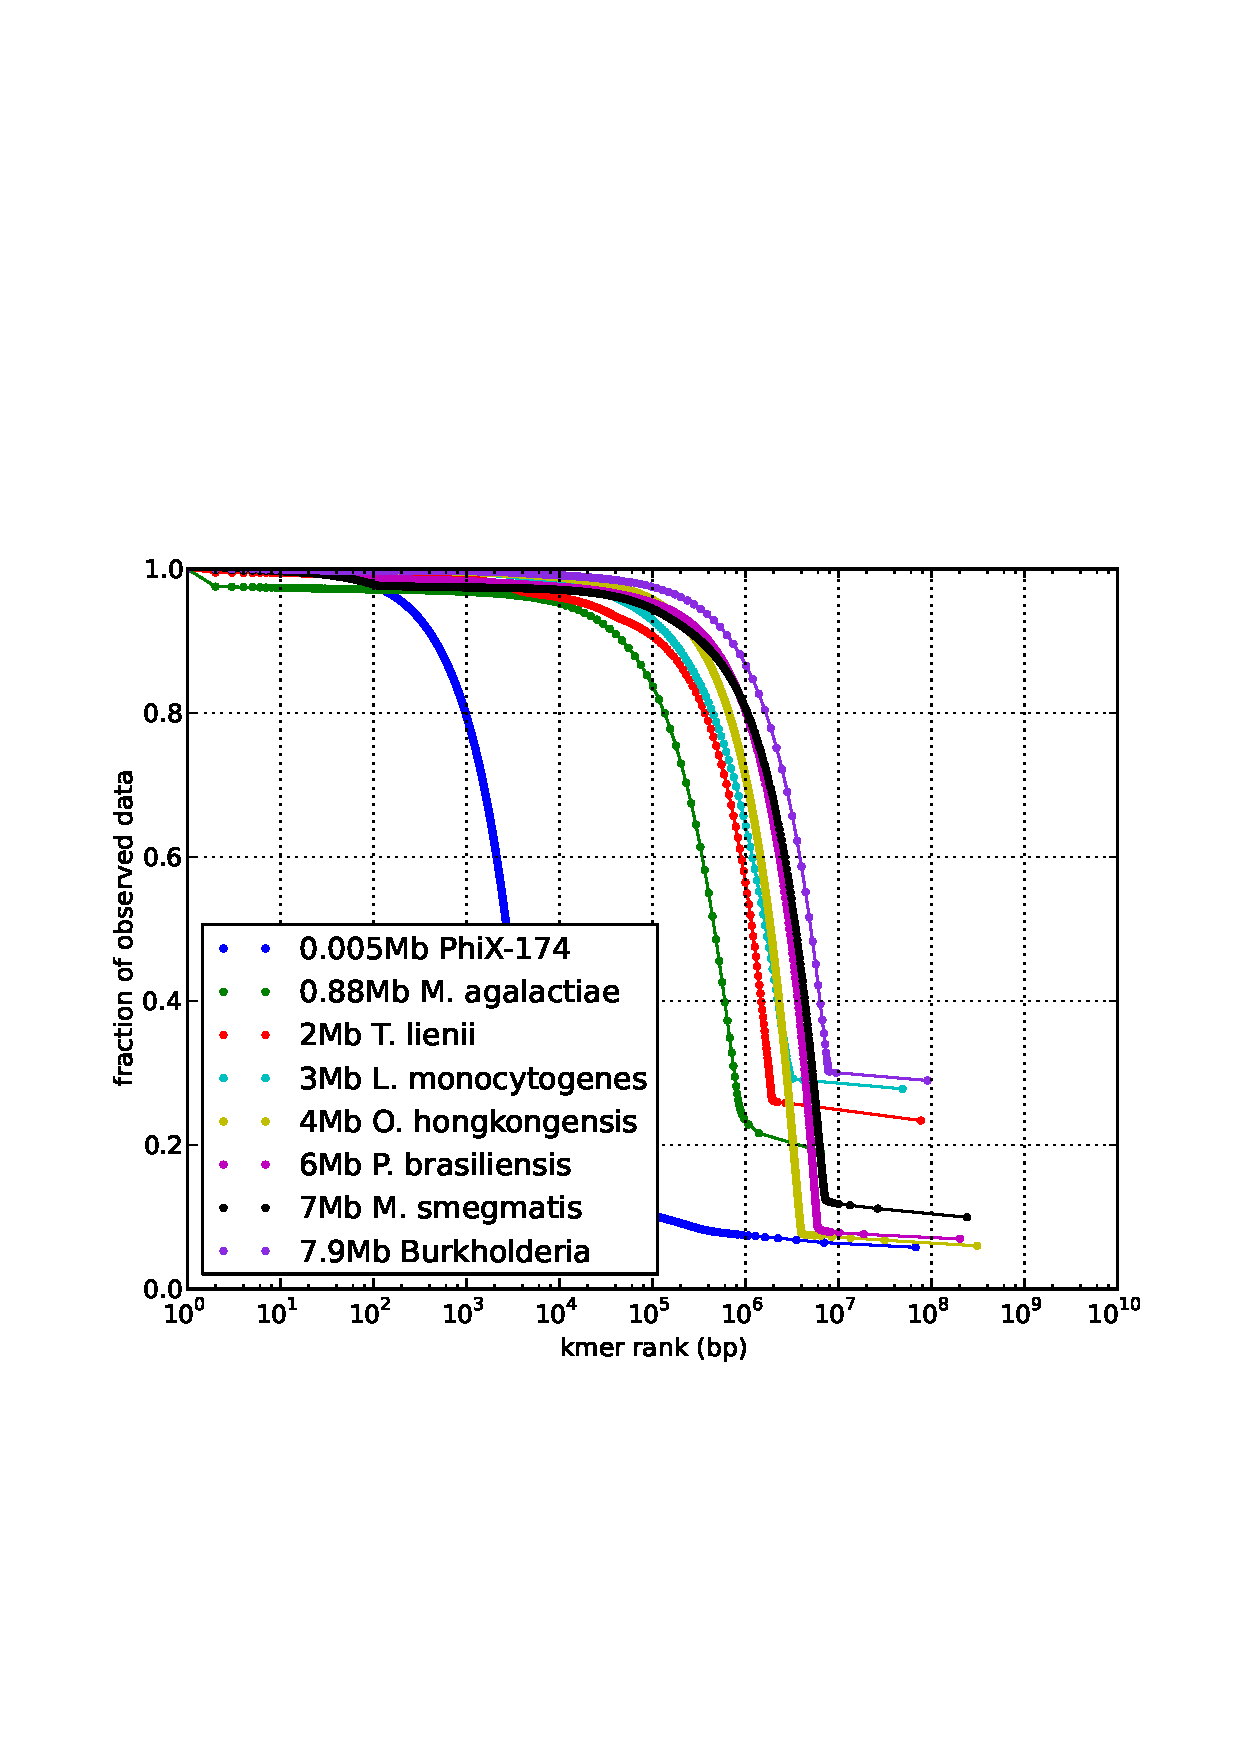
\includegraphics[width=3in]{graphs2/filelistsz-5.pdf}
\end{center}
\caption{Ranked kmer consumed (graph 5).  E. coli is on the left, various genomes are compared on the right. This 
graph shows the fractions of the data in the first $n$ kmers on the horizontal axis.  Here the most highly abundant
kmers are at left and top, rare kmers are on the right and the bottom.}
\label{graph5}
\end{figure}
	
\subsection{Kmer rank abundance (graph 6)}
The kmers can be conceptually ranked from most abundant to least abundant.  This puts the
most abundant kmer first, the 1000th most abundant kmer at position 1000, and the 10 millionth
most abundant kmer in position 10 million.  The plot of the abundance of as a function of rank 
is smoother and can be downsampled for rendering without compromising its meaning.
Additionally, in favorable cases genome size, abundance, and repeat classes can be read from 
this graph.

\begin{figure}
\begin{center}
\includegraphics[width=3in]{graphs3/SRR001665-both-21-6.pdf} 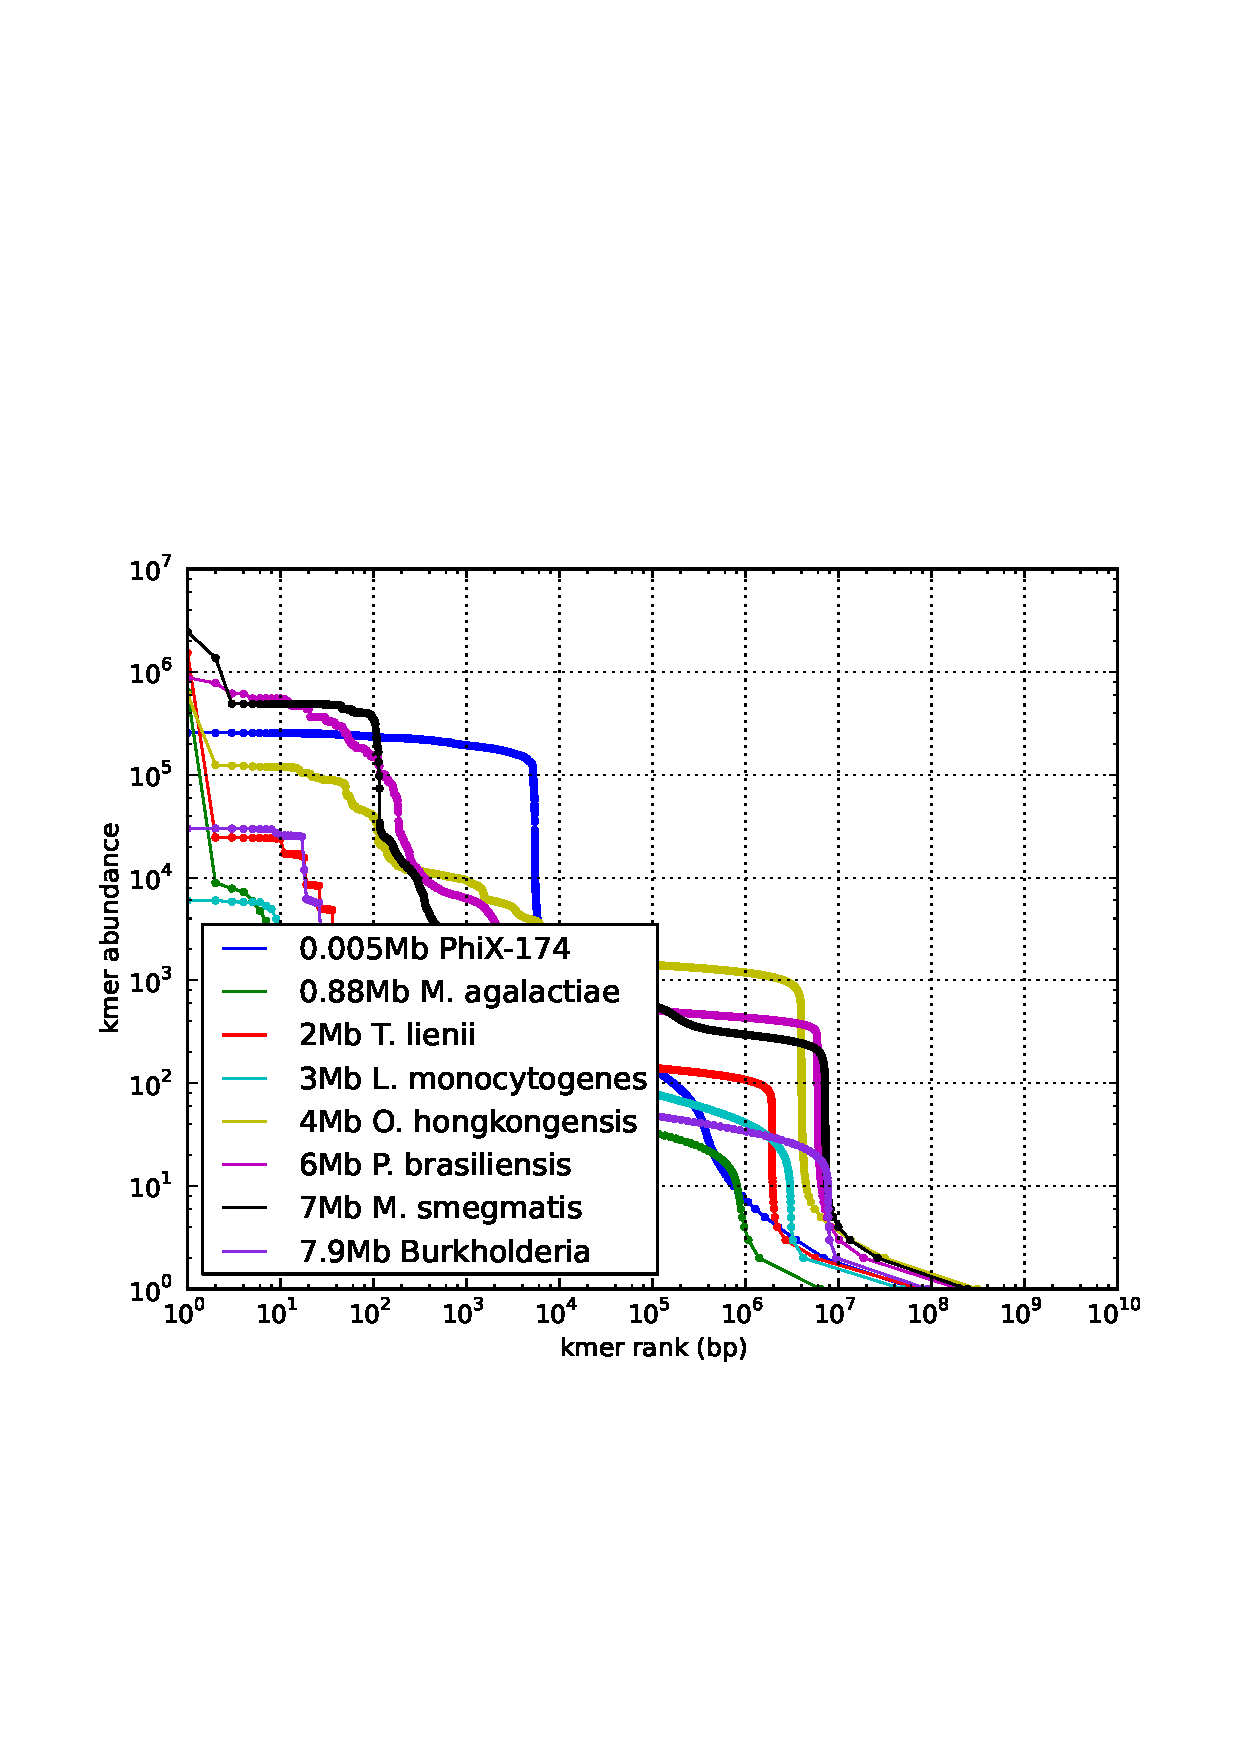
\includegraphics[width=3in]{graphs2/filelistsz-6.pdf}
\end{center}
\caption{Kmer rank abundance (graph 6).  E. Coli is on left, various genomes are compared on right.  This visualization
permits the genome size and kmer abundance to be estimated from the graph; plateaus represent 
uniform-coverage sets of sequences (often genomes).  Note the contrast between 5.4kbase PhiX 
at abundance 170,000 and the multi-megabase genomes at few 100x abundances. }
\label{graph6}
\end{figure}

Plateaus on this graph indicate  collections of kmers at similar levels of abundance.  The
horizontal extent of the plateaus conveys the amount of distinct sequence, while the vertical
position indicates the abundance.

\section{Diagnostic signals}

\begin{itemize}
\item When the F100 statistic is large, this indicates adapter contamination.
F100 approximates the fraction of the dataset that is consumed by adapter sequences,
utilizing the assumption that the most abundant 100 kmers, if highly abundance, 
are likely artifactual sequences.

\item The kink in the Ranked Kmers Consumed (graph 5) graph separates "soild" kmers
(on the left) from "nonsolid" kmers on the right.  
Low accuracy sequencing causes the kink to happen at higher data fractions on the graph.  
This indicates that larger fractions of the dataset lie to the left of the "trough" in 
the kmer abundance graph (graph 1).
High technical-fidelity datasets have no more than a few percent of the data in the
nonsolid kmers.
\item When kmerspectrumanalyzer converges on a genome size with a low ($< 0.1$) shape
factor, the genome size estimate is pretty good.  When kmerspectrumanalyzer converges
with large shape factors, or when the fit fails to converge, this indicates severely
non-uniform genome coverage or other problems.
\item The M50 statistic is about half of the genome size for genome sequencing projects.
\item The AVC statistic should give a good (model-independent) assessment of overall sequencing
depth / effort.
\end{itemize}

\section{Limitations}
\begin{itemize}
\item Very large, diverse input data will exhaust memory in the jellyfish merging step on some machines. 
\item Datasets with very large amounts of adapter contamination ($>$ 10M reads) will overflow the kmer bins
corresponding to the adapter sequences.  This results in inaccurate ratios of
data fraction to total observed kmers, and causes an underestimate of adapter contamination,
but should not otherwise cause problems.  This problem is fairly easy to detect--
if the bin with abundance 10000001 has more than one count, probably indicates overflow.
\item  The underlying model here is much better behaved for those parts of the kmer spectrum
above abundances of, say, 10.  Inferences based on repeatedly observed kmers should
be stronger than any inferences based on the singletons, whose true abundance cannot be 
estimated accurately.
\end{itemize}

\section{Authors and license}
kmerspectrumanalyzer is under the BSD license; see LICENSE.
Distribution, modification and redistribution, incorporation
into other software, and pretty much everything else is allowed.

\begin{itemize}
\item Will Trimble (Argonne National Laboratory)
\item David Williams (Yale University)
\item Travis Harrison (Argonne National Laboratory)
\end{itemize}

A paper describing the genome-size-fitting aspects of kmerspectrumanalyzer was
published August 2013 in BMC Genomics. 2013 14(1):537
"Rapid quantification of sequence repeats to resolve the size, 
structure and contents of bacterial genomes" 
Williams D, Trimble WL, Shilts M, Meyer F, and Ochman H.  PMID: 23924250
The manuscript can be found in repeatresolutionpaper/manuscript and 
the paper at http://www.ncbi.nlm.nih.gov/pmc/articles/PMC3751351

\section{Appendix: edge effect}
We use ``abundance'' to refer to the number of observations of a kmer in a 
dataset and ``coverage'' (sometimes called depth) to refer to the inferred average 
number of reads overlapping each locus in the genome.  The abundances depend on $k$: 
they are biased to lower values than 
the coverage by a factor of $ {L - k + 1} \over {L} $

When overlapping kmers are identified in a sequence, each unambiguous sequence generates 
$$ \textrm{(kmers from read of length L)} = L - k + 1 $$
kmers, so the number of kmers sampled is smaller than the number of base pairs sequenced:
$$\textrm{abundance}_k \approx \textrm{coverage} {{L - k + 1} \over {L}}$$

\bibliography{/Users/wltrimbl/Documents/latex/Ra/Ra}{}
\bibliographystyle{plain}
\end{document}
